% Created by tikzDevice version 0.12 on 2019-05-07 15:15:52
% !TEX encoding = UTF-8 Unicode
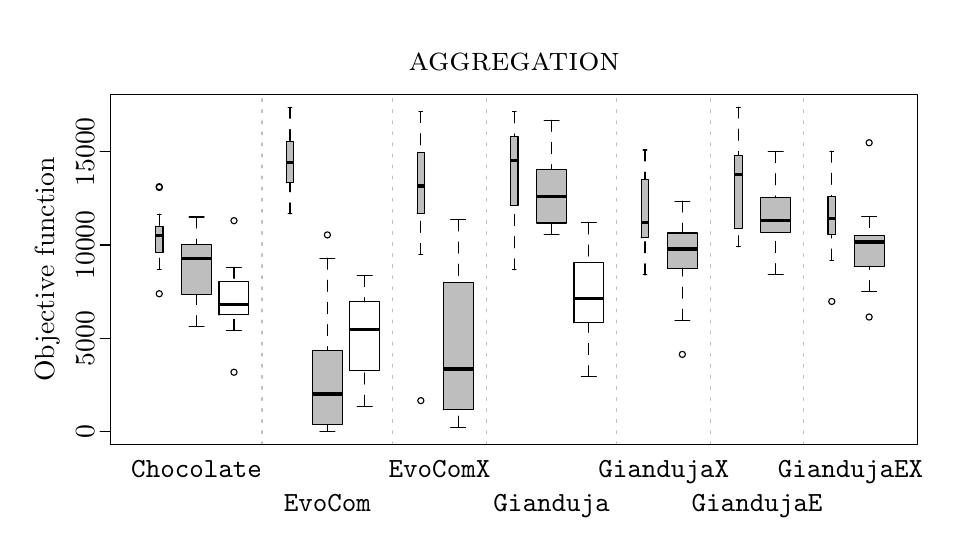
\begin{tikzpicture}[x=1pt,y=1pt]
\definecolor{fillColor}{RGB}{255,255,255}
\path[use as bounding box,fill=fillColor,fill opacity=0.00] (0,0) rectangle (325.21,180.67);
\begin{scope}
\path[clip] ( 30.00, 30.00) rectangle (321.61,156.67);
\definecolor{fillColor}{RGB}{190,190,190}

\path[fill=fillColor] ( 46.20, 99.54) --
	( 48.90, 99.54) --
	( 48.90,108.76) --
	( 46.20,108.76) --
	cycle;
\definecolor{drawColor}{RGB}{0,0,0}

\path[draw=drawColor,line width= 1.2pt,line join=round] ( 46.20,105.45) -- ( 48.90,105.45);

\path[draw=drawColor,line width= 0.4pt,dash pattern=on 4pt off 4pt ,line join=round,line cap=round] ( 47.55, 93.37) -- ( 47.55, 99.54);

\path[draw=drawColor,line width= 0.4pt,dash pattern=on 4pt off 4pt ,line join=round,line cap=round] ( 47.55,113.25) -- ( 47.55,108.76);

\path[draw=drawColor,line width= 0.4pt,line join=round,line cap=round] ( 46.88, 93.37) -- ( 48.23, 93.37);

\path[draw=drawColor,line width= 0.4pt,line join=round,line cap=round] ( 46.88,113.25) -- ( 48.23,113.25);

\path[draw=drawColor,line width= 0.4pt,line join=round,line cap=round] ( 46.20, 99.54) --
	( 48.90, 99.54) --
	( 48.90,108.76) --
	( 46.20,108.76) --
	( 46.20, 99.54);

\path[draw=drawColor,line width= 0.4pt,line join=round,line cap=round] ( 47.55, 84.53) circle (  1.12);

\path[draw=drawColor,line width= 0.4pt,line join=round,line cap=round] ( 47.55,123.22) circle (  1.12);

\path[draw=drawColor,line width= 0.4pt,line join=round,line cap=round] ( 47.55,122.94) circle (  1.12);

\path[fill=fillColor] ( 55.65, 84.30) --
	( 66.45, 84.30) --
	( 66.45,102.25) --
	( 55.65,102.25) --
	cycle;

\path[draw=drawColor,line width= 1.2pt,line join=round] ( 55.65, 97.16) -- ( 66.45, 97.16);

\path[draw=drawColor,line width= 0.4pt,dash pattern=on 4pt off 4pt ,line join=round,line cap=round] ( 61.05, 72.63) -- ( 61.05, 84.30);

\path[draw=drawColor,line width= 0.4pt,dash pattern=on 4pt off 4pt ,line join=round,line cap=round] ( 61.05,112.24) -- ( 61.05,102.25);

\path[draw=drawColor,line width= 0.4pt,line join=round,line cap=round] ( 58.35, 72.63) -- ( 63.75, 72.63);

\path[draw=drawColor,line width= 0.4pt,line join=round,line cap=round] ( 58.35,112.24) -- ( 63.75,112.24);

\path[draw=drawColor,line width= 0.4pt,line join=round,line cap=round] ( 55.65, 84.30) --
	( 66.45, 84.30) --
	( 66.45,102.25) --
	( 55.65,102.25) --
	( 55.65, 84.30);
\definecolor{fillColor}{RGB}{255,255,255}

\path[fill=fillColor] ( 69.15, 76.88) --
	( 79.95, 76.88) --
	( 79.95, 88.86) --
	( 69.15, 88.86) --
	cycle;

\path[draw=drawColor,line width= 1.2pt,line join=round] ( 69.15, 80.73) -- ( 79.95, 80.73);

\path[draw=drawColor,line width= 0.4pt,dash pattern=on 4pt off 4pt ,line join=round,line cap=round] ( 74.55, 71.28) -- ( 74.55, 76.88);

\path[draw=drawColor,line width= 0.4pt,dash pattern=on 4pt off 4pt ,line join=round,line cap=round] ( 74.55, 94.09) -- ( 74.55, 88.86);

\path[draw=drawColor,line width= 0.4pt,line join=round,line cap=round] ( 71.85, 71.28) -- ( 77.25, 71.28);

\path[draw=drawColor,line width= 0.4pt,line join=round,line cap=round] ( 71.85, 94.09) -- ( 77.25, 94.09);

\path[draw=drawColor,line width= 0.4pt,line join=round,line cap=round] ( 69.15, 76.88) --
	( 79.95, 76.88) --
	( 79.95, 88.86) --
	( 69.15, 88.86) --
	( 69.15, 76.88);

\path[draw=drawColor,line width= 0.4pt,line join=round,line cap=round] ( 74.55, 56.16) circle (  1.12);

\path[draw=drawColor,line width= 0.4pt,line join=round,line cap=round] ( 74.55,110.93) circle (  1.12);
\definecolor{fillColor}{RGB}{190,190,190}

\path[fill=fillColor] ( 93.45,124.61) --
	( 96.15,124.61) --
	( 96.15,139.52) --
	( 93.45,139.52) --
	cycle;

\path[draw=drawColor,line width= 1.2pt,line join=round] ( 93.45,132.00) -- ( 96.15,132.00);

\path[draw=drawColor,line width= 0.4pt,dash pattern=on 4pt off 4pt ,line join=round,line cap=round] ( 94.80,113.38) -- ( 94.80,124.61);

\path[draw=drawColor,line width= 0.4pt,dash pattern=on 4pt off 4pt ,line join=round,line cap=round] ( 94.80,151.91) -- ( 94.80,139.52);

\path[draw=drawColor,line width= 0.4pt,line join=round,line cap=round] ( 94.13,113.38) -- ( 95.48,113.38);

\path[draw=drawColor,line width= 0.4pt,line join=round,line cap=round] ( 94.13,151.91) -- ( 95.48,151.91);

\path[draw=drawColor,line width= 0.4pt,line join=round,line cap=round] ( 93.45,124.61) --
	( 96.15,124.61) --
	( 96.15,139.52) --
	( 93.45,139.52) --
	( 93.45,124.61);

\path[fill=fillColor] (102.90, 37.23) --
	(113.70, 37.23) --
	(113.70, 64.06) --
	(102.90, 64.06) --
	cycle;

\path[draw=drawColor,line width= 1.2pt,line join=round] (102.90, 48.35) -- (113.70, 48.35);

\path[draw=drawColor,line width= 0.4pt,dash pattern=on 4pt off 4pt ,line join=round,line cap=round] (108.30, 34.69) -- (108.30, 37.23);

\path[draw=drawColor,line width= 0.4pt,dash pattern=on 4pt off 4pt ,line join=round,line cap=round] (108.30, 97.39) -- (108.30, 64.06);

\path[draw=drawColor,line width= 0.4pt,line join=round,line cap=round] (105.60, 34.69) -- (111.00, 34.69);

\path[draw=drawColor,line width= 0.4pt,line join=round,line cap=round] (105.60, 97.39) -- (111.00, 97.39);

\path[draw=drawColor,line width= 0.4pt,line join=round,line cap=round] (102.90, 37.23) --
	(113.70, 37.23) --
	(113.70, 64.06) --
	(102.90, 64.06) --
	(102.90, 37.23);

\path[draw=drawColor,line width= 0.4pt,line join=round,line cap=round] (108.30,105.79) circle (  1.12);
\definecolor{fillColor}{RGB}{255,255,255}

\path[fill=fillColor] (116.40, 56.73) --
	(127.20, 56.73) --
	(127.20, 81.60) --
	(116.40, 81.60) --
	cycle;

\path[draw=drawColor,line width= 1.2pt,line join=round] (116.40, 71.65) -- (127.20, 71.65);

\path[draw=drawColor,line width= 0.4pt,dash pattern=on 4pt off 4pt ,line join=round,line cap=round] (121.80, 43.91) -- (121.80, 56.73);

\path[draw=drawColor,line width= 0.4pt,dash pattern=on 4pt off 4pt ,line join=round,line cap=round] (121.80, 91.11) -- (121.80, 81.60);

\path[draw=drawColor,line width= 0.4pt,line join=round,line cap=round] (119.10, 43.91) -- (124.50, 43.91);

\path[draw=drawColor,line width= 0.4pt,line join=round,line cap=round] (119.10, 91.11) -- (124.50, 91.11);

\path[draw=drawColor,line width= 0.4pt,line join=round,line cap=round] (116.40, 56.73) --
	(127.20, 56.73) --
	(127.20, 81.60) --
	(116.40, 81.60) --
	(116.40, 56.73);
\definecolor{fillColor}{RGB}{190,190,190}

\path[fill=fillColor] (140.71,113.56) --
	(143.41,113.56) --
	(143.41,135.60) --
	(140.71,135.60) --
	cycle;

\path[draw=drawColor,line width= 1.2pt,line join=round] (140.71,123.42) -- (143.41,123.42);

\path[draw=drawColor,line width= 0.4pt,dash pattern=on 4pt off 4pt ,line join=round,line cap=round] (142.06, 98.71) -- (142.06,113.56);

\path[draw=drawColor,line width= 0.4pt,dash pattern=on 4pt off 4pt ,line join=round,line cap=round] (142.06,150.34) -- (142.06,135.60);

\path[draw=drawColor,line width= 0.4pt,line join=round,line cap=round] (141.38, 98.71) -- (142.73, 98.71);

\path[draw=drawColor,line width= 0.4pt,line join=round,line cap=round] (141.38,150.34) -- (142.73,150.34);

\path[draw=drawColor,line width= 0.4pt,line join=round,line cap=round] (140.71,113.56) --
	(143.41,113.56) --
	(143.41,135.60) --
	(140.71,135.60) --
	(140.71,113.56);

\path[draw=drawColor,line width= 0.4pt,line join=round,line cap=round] (142.06, 45.90) circle (  1.12);

\path[fill=fillColor] (150.16, 42.58) --
	(160.96, 42.58) --
	(160.96, 88.47) --
	(150.16, 88.47) --
	cycle;

\path[draw=drawColor,line width= 1.2pt,line join=round] (150.16, 57.36) -- (160.96, 57.36);

\path[draw=drawColor,line width= 0.4pt,dash pattern=on 4pt off 4pt ,line join=round,line cap=round] (155.56, 36.32) -- (155.56, 42.58);

\path[draw=drawColor,line width= 0.4pt,dash pattern=on 4pt off 4pt ,line join=round,line cap=round] (155.56,111.21) -- (155.56, 88.47);

\path[draw=drawColor,line width= 0.4pt,line join=round,line cap=round] (152.86, 36.32) -- (158.26, 36.32);

\path[draw=drawColor,line width= 0.4pt,line join=round,line cap=round] (152.86,111.21) -- (158.26,111.21);

\path[draw=drawColor,line width= 0.4pt,line join=round,line cap=round] (150.16, 42.58) --
	(160.96, 42.58) --
	(160.96, 88.47) --
	(150.16, 88.47) --
	(150.16, 42.58);

\path[fill=fillColor] (174.46,116.57) --
	(177.16,116.57) --
	(177.16,141.42) --
	(174.46,141.42) --
	cycle;

\path[draw=drawColor,line width= 1.2pt,line join=round] (174.46,132.60) -- (177.16,132.60);

\path[draw=drawColor,line width= 0.4pt,dash pattern=on 4pt off 4pt ,line join=round,line cap=round] (175.81, 93.15) -- (175.81,116.57);

\path[draw=drawColor,line width= 0.4pt,dash pattern=on 4pt off 4pt ,line join=round,line cap=round] (175.81,150.31) -- (175.81,141.42);

\path[draw=drawColor,line width= 0.4pt,line join=round,line cap=round] (175.13, 93.15) -- (176.48, 93.15);

\path[draw=drawColor,line width= 0.4pt,line join=round,line cap=round] (175.13,150.31) -- (176.48,150.31);

\path[draw=drawColor,line width= 0.4pt,line join=round,line cap=round] (174.46,116.57) --
	(177.16,116.57) --
	(177.16,141.42) --
	(174.46,141.42) --
	(174.46,116.57);

\path[fill=fillColor] (183.91,110.08) --
	(194.71,110.08) --
	(194.71,129.38) --
	(183.91,129.38) --
	cycle;

\path[draw=drawColor,line width= 1.2pt,line join=round] (183.91,119.54) -- (194.71,119.54);

\path[draw=drawColor,line width= 0.4pt,dash pattern=on 4pt off 4pt ,line join=round,line cap=round] (189.31,106.06) -- (189.31,110.08);

\path[draw=drawColor,line width= 0.4pt,dash pattern=on 4pt off 4pt ,line join=round,line cap=round] (189.31,147.20) -- (189.31,129.38);

\path[draw=drawColor,line width= 0.4pt,line join=round,line cap=round] (186.61,106.06) -- (192.01,106.06);

\path[draw=drawColor,line width= 0.4pt,line join=round,line cap=round] (186.61,147.20) -- (192.01,147.20);

\path[draw=drawColor,line width= 0.4pt,line join=round,line cap=round] (183.91,110.08) --
	(194.71,110.08) --
	(194.71,129.38) --
	(183.91,129.38) --
	(183.91,110.08);
\definecolor{fillColor}{RGB}{255,255,255}

\path[fill=fillColor] (197.41, 74.03) --
	(208.21, 74.03) --
	(208.21, 95.88) --
	(197.41, 95.88) --
	cycle;

\path[draw=drawColor,line width= 1.2pt,line join=round] (197.41, 82.80) -- (208.21, 82.80);

\path[draw=drawColor,line width= 0.4pt,dash pattern=on 4pt off 4pt ,line join=round,line cap=round] (202.81, 54.56) -- (202.81, 74.03);

\path[draw=drawColor,line width= 0.4pt,dash pattern=on 4pt off 4pt ,line join=round,line cap=round] (202.81,110.12) -- (202.81, 95.88);

\path[draw=drawColor,line width= 0.4pt,line join=round,line cap=round] (200.11, 54.56) -- (205.51, 54.56);

\path[draw=drawColor,line width= 0.4pt,line join=round,line cap=round] (200.11,110.12) -- (205.51,110.12);

\path[draw=drawColor,line width= 0.4pt,line join=round,line cap=round] (197.41, 74.03) --
	(208.21, 74.03) --
	(208.21, 95.88) --
	(197.41, 95.88) --
	(197.41, 74.03);
\definecolor{fillColor}{RGB}{190,190,190}

\path[fill=fillColor] (221.71,104.69) --
	(224.41,104.69) --
	(224.41,125.79) --
	(221.71,125.79) --
	cycle;

\path[draw=drawColor,line width= 1.2pt,line join=round] (221.71,110.26) -- (224.41,110.26);

\path[draw=drawColor,line width= 0.4pt,dash pattern=on 4pt off 4pt ,line join=round,line cap=round] (223.06, 91.33) -- (223.06,104.69);

\path[draw=drawColor,line width= 0.4pt,dash pattern=on 4pt off 4pt ,line join=round,line cap=round] (223.06,136.47) -- (223.06,125.79);

\path[draw=drawColor,line width= 0.4pt,line join=round,line cap=round] (222.38, 91.33) -- (223.73, 91.33);

\path[draw=drawColor,line width= 0.4pt,line join=round,line cap=round] (222.38,136.47) -- (223.73,136.47);

\path[draw=drawColor,line width= 0.4pt,line join=round,line cap=round] (221.71,104.69) --
	(224.41,104.69) --
	(224.41,125.79) --
	(221.71,125.79) --
	(221.71,104.69);

\path[fill=fillColor] (231.16, 93.75) --
	(241.96, 93.75) --
	(241.96,106.47) --
	(231.16,106.47) --
	cycle;

\path[draw=drawColor,line width= 1.2pt,line join=round] (231.16,100.65) -- (241.96,100.65);

\path[draw=drawColor,line width= 0.4pt,dash pattern=on 4pt off 4pt ,line join=round,line cap=round] (236.56, 74.91) -- (236.56, 93.75);

\path[draw=drawColor,line width= 0.4pt,dash pattern=on 4pt off 4pt ,line join=round,line cap=round] (236.56,118.01) -- (236.56,106.47);

\path[draw=drawColor,line width= 0.4pt,line join=round,line cap=round] (233.86, 74.91) -- (239.26, 74.91);

\path[draw=drawColor,line width= 0.4pt,line join=round,line cap=round] (233.86,118.01) -- (239.26,118.01);

\path[draw=drawColor,line width= 0.4pt,line join=round,line cap=round] (231.16, 93.75) --
	(241.96, 93.75) --
	(241.96,106.47) --
	(231.16,106.47) --
	(231.16, 93.75);

\path[draw=drawColor,line width= 0.4pt,line join=round,line cap=round] (236.56, 62.61) circle (  1.12);

\path[fill=fillColor] (255.46,108.03) --
	(258.16,108.03) --
	(258.16,134.53) --
	(255.46,134.53) --
	cycle;

\path[draw=drawColor,line width= 1.2pt,line join=round] (255.46,127.50) -- (258.16,127.50);

\path[draw=drawColor,line width= 0.4pt,dash pattern=on 4pt off 4pt ,line join=round,line cap=round] (256.81,101.51) -- (256.81,108.03);

\path[draw=drawColor,line width= 0.4pt,dash pattern=on 4pt off 4pt ,line join=round,line cap=round] (256.81,151.98) -- (256.81,134.53);

\path[draw=drawColor,line width= 0.4pt,line join=round,line cap=round] (256.14,101.51) -- (257.49,101.51);

\path[draw=drawColor,line width= 0.4pt,line join=round,line cap=round] (256.14,151.98) -- (257.49,151.98);

\path[draw=drawColor,line width= 0.4pt,line join=round,line cap=round] (255.46,108.03) --
	(258.16,108.03) --
	(258.16,134.53) --
	(255.46,134.53) --
	(255.46,108.03);

\path[fill=fillColor] (264.91,106.81) --
	(275.71,106.81) --
	(275.71,119.24) --
	(264.91,119.24) --
	cycle;

\path[draw=drawColor,line width= 1.2pt,line join=round] (264.91,110.88) -- (275.71,110.88);

\path[draw=drawColor,line width= 0.4pt,dash pattern=on 4pt off 4pt ,line join=round,line cap=round] (270.31, 91.41) -- (270.31,106.81);

\path[draw=drawColor,line width= 0.4pt,dash pattern=on 4pt off 4pt ,line join=round,line cap=round] (270.31,135.89) -- (270.31,119.24);

\path[draw=drawColor,line width= 0.4pt,line join=round,line cap=round] (267.61, 91.41) -- (273.01, 91.41);

\path[draw=drawColor,line width= 0.4pt,line join=round,line cap=round] (267.61,135.89) -- (273.01,135.89);

\path[draw=drawColor,line width= 0.4pt,line join=round,line cap=round] (264.91,106.81) --
	(275.71,106.81) --
	(275.71,119.24) --
	(264.91,119.24) --
	(264.91,106.81);

\path[fill=fillColor] (289.21,105.90) --
	(291.91,105.90) --
	(291.91,119.68) --
	(289.21,119.68) --
	cycle;

\path[draw=drawColor,line width= 1.2pt,line join=round] (289.21,111.67) -- (291.91,111.67);

\path[draw=drawColor,line width= 0.4pt,dash pattern=on 4pt off 4pt ,line join=round,line cap=round] (290.56, 96.68) -- (290.56,105.90);

\path[draw=drawColor,line width= 0.4pt,dash pattern=on 4pt off 4pt ,line join=round,line cap=round] (290.56,136.05) -- (290.56,119.68);

\path[draw=drawColor,line width= 0.4pt,line join=round,line cap=round] (289.89, 96.68) -- (291.24, 96.68);

\path[draw=drawColor,line width= 0.4pt,line join=round,line cap=round] (289.89,136.05) -- (291.24,136.05);

\path[draw=drawColor,line width= 0.4pt,line join=round,line cap=round] (289.21,105.90) --
	(291.91,105.90) --
	(291.91,119.68) --
	(289.21,119.68) --
	(289.21,105.90);

\path[draw=drawColor,line width= 0.4pt,line join=round,line cap=round] (290.56, 81.74) circle (  1.12);

\path[fill=fillColor] (298.66, 94.52) --
	(309.46, 94.52) --
	(309.46,105.71) --
	(298.66,105.71) --
	cycle;

\path[draw=drawColor,line width= 1.2pt,line join=round] (298.66,103.24) -- (309.46,103.24);

\path[draw=drawColor,line width= 0.4pt,dash pattern=on 4pt off 4pt ,line join=round,line cap=round] (304.06, 85.30) -- (304.06, 94.52);

\path[draw=drawColor,line width= 0.4pt,dash pattern=on 4pt off 4pt ,line join=round,line cap=round] (304.06,112.42) -- (304.06,105.71);

\path[draw=drawColor,line width= 0.4pt,line join=round,line cap=round] (301.36, 85.30) -- (306.76, 85.30);

\path[draw=drawColor,line width= 0.4pt,line join=round,line cap=round] (301.36,112.42) -- (306.76,112.42);

\path[draw=drawColor,line width= 0.4pt,line join=round,line cap=round] (298.66, 94.52) --
	(309.46, 94.52) --
	(309.46,105.71) --
	(298.66,105.71) --
	(298.66, 94.52);

\path[draw=drawColor,line width= 0.4pt,line join=round,line cap=round] (304.06, 76.11) circle (  1.12);

\path[draw=drawColor,line width= 0.4pt,line join=round,line cap=round] (304.06,139.09) circle (  1.12);
\definecolor{drawColor}{RGB}{190,190,190}

\path[draw=drawColor,line width= 0.4pt,dash pattern=on 1pt off 3pt ,line join=round,line cap=round] ( 84.68, 30.00) -- ( 84.68,156.67);

\path[draw=drawColor,line width= 0.4pt,dash pattern=on 1pt off 3pt ,line join=round,line cap=round] (131.93, 30.00) -- (131.93,156.67);

\path[draw=drawColor,line width= 0.4pt,dash pattern=on 1pt off 3pt ,line join=round,line cap=round] (165.68, 30.00) -- (165.68,156.67);

\path[draw=drawColor,line width= 0.4pt,dash pattern=on 1pt off 3pt ,line join=round,line cap=round] (212.93, 30.00) -- (212.93,156.67);

\path[draw=drawColor,line width= 0.4pt,dash pattern=on 1pt off 3pt ,line join=round,line cap=round] (246.69, 30.00) -- (246.69,156.67);

\path[draw=drawColor,line width= 0.4pt,dash pattern=on 1pt off 3pt ,line join=round,line cap=round] (280.44, 30.00) -- (280.44,156.67);
\end{scope}
\begin{scope}
\path[clip] (  0.00,  0.00) rectangle (325.21,180.67);
\definecolor{drawColor}{RGB}{0,0,0}

\node[text=drawColor,anchor=base,inner sep=0pt, outer sep=0pt, scale=  1.00] at ( 61.05, 18.00) {\texttt{Chocolate}};

\node[text=drawColor,anchor=base,inner sep=0pt, outer sep=0pt, scale=  1.00] at (148.81, 18.00) {\texttt{EvoComX}};

\node[text=drawColor,anchor=base,inner sep=0pt, outer sep=0pt, scale=  1.00] at (229.81, 18.00) {\texttt{GiandujaX}};

\node[text=drawColor,anchor=base,inner sep=0pt, outer sep=0pt, scale=  1.00] at (297.31, 18.00) {\texttt{GiandujaEX}};

\node[text=drawColor,anchor=base,inner sep=0pt, outer sep=0pt, scale=  1.00] at (108.30,  6.00) {\texttt{EvoCom}};

\node[text=drawColor,anchor=base,inner sep=0pt, outer sep=0pt, scale=  1.00] at (189.31,  6.00) {\texttt{Gianduja}};

\node[text=drawColor,anchor=base,inner sep=0pt, outer sep=0pt, scale=  1.00] at (263.56,  6.00) {\texttt{GiandujaE}};
\end{scope}
\begin{scope}
\path[clip] (  0.00,  0.00) rectangle (325.21,180.67);
\definecolor{drawColor}{RGB}{0,0,0}

\node[text=drawColor,anchor=base,inner sep=0pt, outer sep=0pt, scale=  1.20] at (175.81,165.07) {\textsc{aggregation}};

\node[text=drawColor,rotate= 90.00,anchor=base,inner sep=0pt, outer sep=0pt, scale=  1.00] at (  9.60, 93.34) {Objective function};
\end{scope}
\begin{scope}
\path[clip] (  0.00,  0.00) rectangle (325.21,180.67);
\definecolor{drawColor}{RGB}{0,0,0}

\path[draw=drawColor,line width= 0.4pt,line join=round,line cap=round] ( 30.00, 34.69) -- ( 30.00,135.83);

\path[draw=drawColor,line width= 0.4pt,line join=round,line cap=round] ( 30.00, 34.69) -- ( 26.20, 34.69);

\path[draw=drawColor,line width= 0.4pt,line join=round,line cap=round] ( 30.00, 68.41) -- ( 26.20, 68.41);

\path[draw=drawColor,line width= 0.4pt,line join=round,line cap=round] ( 30.00,102.12) -- ( 26.20,102.12);

\path[draw=drawColor,line width= 0.4pt,line join=round,line cap=round] ( 30.00,135.83) -- ( 26.20,135.83);

\node[text=drawColor,rotate= 90.00,anchor=base,inner sep=0pt, outer sep=0pt, scale=  1.00] at ( 24.00, 34.69) {0};

\node[text=drawColor,rotate= 90.00,anchor=base,inner sep=0pt, outer sep=0pt, scale=  1.00] at ( 24.00, 68.41) {5000};

\node[text=drawColor,rotate= 90.00,anchor=base,inner sep=0pt, outer sep=0pt, scale=  1.00] at ( 24.00,102.12) {10000};

\node[text=drawColor,rotate= 90.00,anchor=base,inner sep=0pt, outer sep=0pt, scale=  1.00] at ( 24.00,135.83) {15000};

\path[draw=drawColor,line width= 0.4pt,line join=round,line cap=round] ( 30.00, 30.00) --
	(321.61, 30.00) --
	(321.61,156.67) --
	( 30.00,156.67) --
	( 30.00, 30.00);
\end{scope}
\end{tikzpicture}
